\chapter{Appendiks} \label{cha:AppC} 
\section{Indkøb af lægemidler}
Indkøb af lægemidler til distribution til de nordjyske hospitaler foretages af Sygehusapoteket Region Nordjylland (SRN)~\citep{SygehusapoteketRegionNordjylland2013}. Salg til Region Nordjyllands (RN) egne institutioner udgør 98,4~\% af det samlede salg i år 2012, hvor under 1~\% går til andre regioners sygehusapoteker og til private apoteker samt andre kunder. Udover indkøb yder SRN information og tilbyder tjenesteydelser til de kliniske afsnit, herunder klinisk farmaci.~\citep{SygehusapoteketRegionNordjylland2013}

Størstedelen af medicinindkøb i år 2012, svarende til 95~\%, skete via. Amgros. Yderligere blev 2~\% købt af andre sygehusapoteker, 1~\% fra private apoteker og 2~\% fra øvrige. ~\citep{SygehusapoteketRegionNordjylland2013}
Bestilling af medicin fra hospitalsafsnittene sker via medicinservice varetaget af farmakonomer. Der bestilles medicin via ApoVision-Online. SRN forgår som lagerholder og fremtager medicin manuelt fra henholdsvis almindeligt hyldelager, pater Noster (halvautomatik lager-reol) og høj-lager (paller).~\citep{SygehusapoteketRegionNordjylland2013}

SRN er opdelt i forskellige afdelinger herunder ledelse, administration, lægemiddelinformation, klinisk farmaci, logistik, kvalitetsafdeling og produktion. De primære aktører ved Amgrosudbud i RN er Amgros-ansvalige, Specialistfarmaceut/ATC-asnarlige og Lægemiddelinformation. Opgaver for disse aktører fremgår af figur\ref{fig:SRNudbud}.

\begin{figure}[H]\centering
	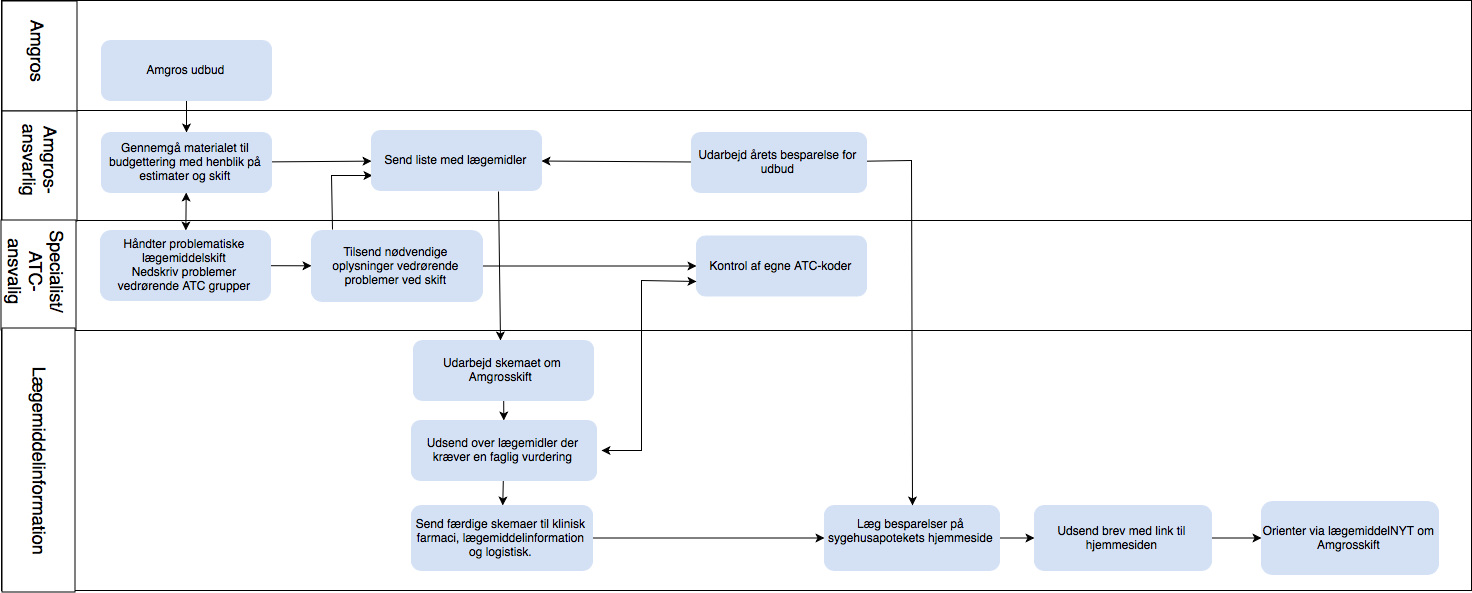
\includegraphics[width=1\textwidth]{billeder/SRNudbud.png} 
	\caption{...}
	\label{fig:SRNudbud}  
\end{figure}

Ved Amgrosudbud står den Amgros-ansvalige  for at gennemgå udbudsmaterialet og budgettestimere i forbindelse med kommende kontrakter. I sammenhæng med dette håndteres problematiske lægemiddelskift af specialist/ATC-ansvarlige. De problemer der vedrører ATC-grupper nedskrives og sendes tilbage til den Amgros-ansvarlige. Den Amgros-ansvarlige sender herefter en liste ud med lægemidler til Lægemiddelinformation, hvorefter der udarbejdes et skema om lægemiddelskift. Lægemiddelinformation udsender herefter en liste med lægemidler der kræver en faglig vurdering til Specialistfarmaceut/ATC-asnarlige, som kontrollere egne ATC-koder. Herefter sendes færdige skemaer til Klinisk farmaci, Lægemiddelinformationen og Logistik i SRN. Dernæst udarbejdes årets samlede besparelse af Amgros-ansvarlige og ligges på Sygehusapotekets hjemmeside af Lægemiddelinformationen som også sender brev med link til hjemmesiden og orientere via LægemiddelNyt omkring Amgrosskift. 